%%%%%%%%%%%%%%%%%%%%%%%%%%%%%%%%%%%%%%%%%%%%%%%%%%%%%%%%%%%%%%%%%%%%%%%%%%%%
% radical_root_en.tex
%
% Compile with XeLaTeX, then BibTeX, followed by two XeLaTeX runs.
%
% Logical scope.  This paper separates a convention (the fractional-power
% collapse on the positive reals), exact structural theorems (the torsion
% split of the power map into quotient and section), and machine-checked
% formalization and computation.  All theorems of the main deduction are
% mechanically verified; nothing is left as an open conjecture.
%%%%%%%%%%%%%%%%%%%%%%%%%%%%%%%%%%%%%%%%%%%%%%%%%%%%%%%%%%%%%%%%%%%%%%%%%%%%

\documentclass[submission,noinfoline]{jsfds}
\usepackage[T1]{fontenc}
\usepackage{amsmath,amsthm,amssymb}
\usepackage{graphicx}
\usepackage[numbers]{natbib}
\usepackage{hyperref}
\makeatletter\let\hy@frontmatter\relax\makeatother
\setlength{\emergencystretch}{2em}
\bibliographystyle{unsrt}

\graphicspath{{figures/}}

\startlocaldefs
\newtheorem{theorem}{Theorem}
\newtheorem{proposition}[theorem]{Proposition}
\newtheorem{corollary}[theorem]{Corollary}
\newtheorem{lemma}[theorem]{Lemma}
\newtheorem{definition}[theorem]{Definition}
\newtheorem*{remark}{Remark}
\setattribute{title}{size}{\LARGE\bfseries}
% Lean identifiers remain in the source as cross-references, but are not printed.
\newcommand{\Lean}[1]{}
\def\journal@name{}%
\setattribute{infoline}{text}{}%
\setattribute{copyright}{text}{}
\newcommand{\abs}[1]{\lvert #1\rvert}
\newcommand{\Norm}[1]{\lVert #1\rVert}
\endlocaldefs

\setmainlanguageenglish
\AtBeginDocument{\renewcommand{\refname}{References}}
\firstpage{1}
\begin{document}
\begin{frontmatter}

\title{The radical as a forced structure:
how to split powers from radicals}
\runtitle{Splitting powers from radicals}

\begin{aug}
  \auteur{%
    \prenom{Yuanjie}
    \nom{Liu}}
  \affiliation{Independent Researcher;\quad
  \href{mailto:yuanjieliu65@gmail.com}{yuanjieliu65@gmail.com}}
  \runauthor{Yuanjie Liu}
\end{aug}

\begin{abstract}
The $n$-th root is commonly regarded as a value of the power family:
$x^{1/n}=x^t$ at $t=1/n$. On the positive reals the collapse is
correct: there $p_n\colon x\mapsto x^n$ is an automorphism and its
inverse is single-valued. We show the collapse is a torsion phenomenon:
it holds precisely where the $n$-th roots of unity are trivial. Over
every commutative group the kernel of the power map is the subgroup
$\mu_n=\{x:x^n=1\}$, every fiber is the coset $x\cdot\mu_n$, and the
radical is not a function but a section of the $n$-fold cover: a choice
among $n$ branches differing by multiplication with $\mu_n$. The
collapse criterion --- $p_n$ is injective if and only if $\mu_n$ is
trivial --- marks where the identification of roots with fractional
powers survives. Three elementary theorems express this split (kernel,
fibers, collapse criterion) and are machine-verified in Lean~4 with
Mathlib: zero proof gaps. Computationally we give certified radical
values and a quadratic solver: $x^2-bx-c=0$ has a real root if and only
if $b^2+4c\ge0$, and both radical roots are exhibited and the polynomial
factors. It climbs to the cubic: the Cardano construction exhibits a
real root of $x^3+px+q=0$ whenever $(q/2)^2+(p/3)^3\ge0$, resting on
surjectivity of the cube map on $\mathbb R$ --- the intermediate value
theorem. It then widens instead of climbing: $\sqrt[n]{x}=\exp(\ln x/n)$
is the unique positive solution of $y^n=x$ for every natural degree, so
quintic roots and roots of every degree are one statement, not a
ladder. Degree five withholds not the pure root but the mixed tower;
solvability of the general quintic by radicals is cited (Abel--Ruffini),
not proved here. Every statement of the main deduction is
machine-checked, and the boundary between executable integer arithmetic
and certified, non-executable real statements is explicit: reductions
over $\mathbb R$ are certified theorems, not computed numeric
iterations.
\end{abstract}

\begin{keywords}
\kwd{radical function}
\kwd{power map}
\kwd{roots of unity}
\kwd{torsion}
\kwd{quotient and section}
\kwd{formal verification}
\end{keywords}

\begin{AMSclass}
\kwd{12F10}
\kwd{03B35}
\kwd{26A09}
\end{AMSclass}
\end{frontmatter}

\begin{quote}
  \itshape ``Eternity is a long time.''
  \par\vspace{2pt}
  \begin{flushright}
    \small --- Isaac Asimov, \emph{Foundation}
  \end{flushright}
\end{quote}
\vspace{0.8em}

\section{Question, inputs, and logical order}\label{sec:intro}

For $t\in\mathbb R$ and $x>0$ the power $x^t=\exp(t\ln x)$
\citep{Euler1748} is a function of two arguments, single-valued, and
nothing prevents evaluating it at $t=1/n$. This yields the received
convention
\begin{equation}
  \text{``the $n$-th root is the fractional power $x^{1/n}$,
  i.e.\ $x^t$ at $t=1/n$''}.
\end{equation}
On the positive reals the convention looks harmless, and is harmless: the
power map $p_n\colon x\mapsto x^n$ is strictly increasing, hence
injective; as a group endomorphism of $\mathbb R_+$ it is an
automorphism, and its inverse is exactly the value of (1). No choice is
ever made, because $\exp$ and $\ln$ are functions, not relations.

The convention answers, before it is asked, the question of how to
invert the map $x\mapsto x^n$. This paper asks where that inversion
fails, and which structure the failure forces into existence. Over a
general multiplicative structure $p_n$ is not injective, and for a group
homomorphism injectivity is equivalent to a trivial kernel. The kernel
of $p_n$ is the subgroup of $n$-th roots of unity,
$\mu_n=\{x:x^n=1\}$; over $\mathbb C^\times$ it is a cyclic group of
order $n$ \citep{Gauss1801}. The failure is not a defect of one formula;
it is measured by $\mu_n$. Once $\mu_n$ is present, the fiber of $p_n$
over $x^n$ is the whole coset $x\cdot\mu_n$, and the symbol $x^{1/n}$,
if it names anything, names a choice among $n$ preimages. Inverting
powers therefore forces three objects into existence: the subgroup
$\mu_n$ that is the kernel, the cosets that are the fibers, and the
sections --- the branch choices --- that textbooks write as roots. The
radical is a section of an $n$-fold cover, not a function.

The main results can be stated without machinery, and we state them now;
proofs follow in the sections indicated.

\begin{itemize}
\item \emph{The torsion split.} For every commutative group $G$ and every
$n$, the kernel of $p_n$ is exactly $\mu_n(G)$
(Theorem~\ref{thm:ker}), every fiber of $p_n$ is the coset
$x\cdot\mu_n(G)$ (Theorem~\ref{thm:fiber}), and $p_n$ is injective if
and only if $\mu_n(G)$ is trivial (Theorem~\ref{thm:collapse}). The
identification (1) survives exactly where the last criterion holds;
over $\mathbb R_+$ it holds because $\mathbb R_+$ is torsion-free. All
three theorems are machine-verified in Lean~4 with Mathlib, zero proof
gaps.
\item \emph{A certified solver ladder.} Over $\mathbb R$ the programme
is certified inside the proof system. For real $b,c$, the equation
$x^2-bx-c=0$ has a real root if and only if $\Delta=b^2+4c\ge0$; when
it does, both radical roots are exhibited and the polynomial factors
(Theorem~\ref{thm:quad}). The ladder climbs to the cubic: whenever
$(q/2)^2+(p/3)^3\ge0$ the Cardano construction exhibits a real root of
$x^3+px+q=0$, with surjectivity of the cube map as its only analytic
input (Theorem~\ref{thm:cubic}). The ladder then stops climbing and
widens: one statement, $\sqrt[n]{x}=\exp(\ln x/n)$, is the unique
positive solution of $y^n=x$ for every degree $n$ at once
(Theorem~\ref{thm:anydegree}). There is no separate quintic theorem.
\item \emph{Where the wall is.} Pure $n$-th roots exist for every
degree. What withholds at degree five is the mixed tower: a general
quintic is not solvable by field operations and extraction of roots of
arbitrary degree. That statement (Abel--Ruffini \citep{Abel1824}, in the
Galois formulation \citep{Galois1846}) is cited as the boundary of this
paper, not proved here; its formalization is not claimed.
\end{itemize}

The strategy is uniform. On $\mathbb R_+$ every power and radical is
constructed from $\ln$ and $\exp$, and there $p_n$ is an automorphism,
so (1) holds verbatim. Over an arbitrary commutative group no analytic
tools exist, and the proofs reduce to the ring identity
$(xy)^n=x^ny^n$ and its consequences: kernel, fibers, collapse
criterion. The certified solvers split the same way. After the
substitution $(\sqrt\Delta)^2=\Delta$ the quadratic is pure algebra,
factorizing $x^2-bx-c=(x-r_+)(x-r_-)$, and the negative-discriminant
case is completing the square; the cubic needs exactly one analytic
input, surjectivity of the cube map on $\mathbb R$ --- Mathlib's
intermediate value theorem --- after which the Cardano identity is again
pure algebra. The entire deduction contains one intermediate-value
argument.

A boundary is kept explicit throughout, between what is proved inside
the proof system and what is cited. Inside: the three structure
theorems, the radical examples, and the quadratic, cubic, and
every-degree theorems are formalized in Lean~4 \citep{deMoura2015} with
Mathlib \citep{MathlibCommunity2020}, in the module
\texttt{Nods.Theories.\allowbreak Radical} of the NODS repository; the module is in
the main build, and a search over the source tree confirms zero
\texttt{sorry}. Cited, not re-proved: the classical context of roots of
unity \citep{Gauss1801}, the provenance of the Cardano construction
\citep{Cardano1545}, and the Abel--Ruffini and Galois statements about
mixed towers \citep{Abel1824,Galois1846}. On the reals, arithmetic is
certified, not executed: $\sqrt{\,}$ is defined by completeness and is
not executable, and reductions such as $\sqrt{16}=4$ via
$\sqrt{a^2}=\abs a$ are certified theorems, not numeric iteration. We
claim certified radical statements, not a numeric radical evaluator.

The order of the paper follows the questions just raised.
Section~\ref{sec:setting} fixes the two objects, the power map and the
subgroup of roots of unity, over an arbitrary commutative group.
Section~\ref{sec:collapse} records the collapse on $\mathbb R_+$ and
its failure over $\mathbb C^\times$. Section~\ref{sec:quotient} states
and proves the three structure theorems --- kernel, fibers as cosets,
collapse criterion --- and reads them as quotient and section.
Section~\ref{sec:numbers} draws the concrete consequence for a single
number. Section~\ref{sec:computation} gives the certified quadratic
solver, the Cardano cubic, and the radical of every degree, and states
the two boundaries (executability, and the degree-five wall against
mixed towers). Section~\ref{sec:formal} records the formalization
choices, and Section~\ref{sec:conclusion} closes.

\subsection{Related work}

The literature this paper touches is old and settled; the contribution
is not new mathematics but a certified statement of where a convention
holds. Roots of unity were studied systematically by Gauss
\citep{Gauss1801}; the impossibility of solving the general quintic by
radicals was proved by Abel \citep{Abel1824}, and Galois turned the
obstruction into group theory \citep{Galois1846}. Fractional powers and
the exponential--logarithm calculus that make $x^{1/n}$ a function on
$\mathbb R_+$ are Euler's \citep{Euler1748}. The cubic solution
certified here goes back to Cardano's \emph{Ars Magna}
\citep{Cardano1545}. On the formal side, Lean \citep{deMoura2015} and
its mathematical library Mathlib \citep{MathlibCommunity2020} supply the
real analysis --- $\exp$, $\ln$, $\sqrt{\,}$, the intermediate value
theorem --- that the certified statements reuse rather than rebuild.

\begin{itemize}
\item Classical radical algebra asks which equations are solvable by
adjoining roots; we ask the narrower question, for one power map, what
its kernel is and what its sections are, and answer it for every
commutative group.
\item Euler's $x^{1/n}$ is correct on $\mathbb R_+$ not because of any
special property of $\exp$, but because $\mu_n\cap\mathbb R_+=1$; the
analysis here locates the reason in torsion.
\item The Cardano construction is four centuries old;
Theorem~\ref{thm:cubic} adds certification and makes explicit a third
appearance of the torsion split --- $v$ cannot be chosen as an
independent cube root.
\item Mathlib already contains real roots and powers; the contribution
of the present module is the splitting statements (kernel, fibers,
collapse criterion over arbitrary commutative groups) and the certified
solvers, with zero proof gaps.
\item Abel--Ruffini and Galois remain cited, not formalized; the
boundary between executable integer arithmetic and certified,
non-executable real statements is stated, not erased.
\end{itemize}

\section{Setting: power maps and roots of unity}\label{sec:setting}

Fix a commutative group $G$, written multiplicatively, and $n\in\mathbb N$.
We use two objects.

\begin{definition}[Power map]\label{def:power}
$p_n\colon G\to G$ denotes $p_n(x)=x^n$.
\end{definition}
\begin{definition}[Roots of unity]\label{def:mu}
$\mu_n(G)=\{x\in G:x^n=1\}$ is the subgroup of $n$-th roots of unity.
\end{definition}

That $\mu_n(G)$ is a subgroup is immediate from commutativity
($(xy)^n=x^ny^n$) and from $(x^{-1})^n=(x^n)^{-1}$. Its elements are
the \emph{torsion} of exponent $n$; $\mu_n(G)=\{1\}$ is the statement that
$G$ has no nontrivial $n$-th root of unity.

$p_n$ is a group homomorphism: $p_n(xy)=(xy)^n=x^ny^n=p_n(x)p_n(y)$,
again by commutativity.

\textbf{Two base groups.} Two instances of the setup run through the
paper. On $G=\mathbb R_+$, the multiplicative group of positive reals,
the equation $x^n=1$ forces $x=1$, so $\mu_n(\mathbb R_+)=\{1\}$: the
roots of unity are trivial, the group is torsion-free. On
$G=\mathbb C^\times$ the same subgroup is the regular $n$-gon
$\mu_n(\mathbb C^\times)=\{e^{2\pi i k/n}:0\le k<n\}$, a cyclic group
with $n$ elements \citep{Gauss1801}. Abstractly, cardinality is never
needed: the theorems of Section~\ref{sec:quotient} are stated for an
arbitrary commutative $G$ and never count roots of unity. That
$\mu_n(\mathbb C^\times)$ has exactly $n$ elements is a concrete fact
about the complex exponential, not an input to the mechanism; on
$\mathbb R_+$ the same subgroup is trivial, and that single fact is the
whole difference between the two worlds.

\textbf{Worked micro-example ($n=2$).} On $G=\mathbb C^\times$,
$\mu_2=\{1,-1\}$, and the fiber of $p_2$ over $x^2$ is $\{x,-x\}$:
both leaves square to $x^2$, and nothing in the group prefers one over
the other. The square root of $x^2$ is therefore a two-element choice;
the two values differ by the kernel element $-1$. On $G=\mathbb R_+$
the contrast is sharp: for $x>0$ the fiber over $x^2$ is the singleton
$\{x\}$, since $-x\notin\mathbb R_+$. The two-element choice collapses
to one element, $\sqrt{x^2}=x$ is forced, and the collapse of
Section~\ref{sec:collapse} is already visible here in its simplest
form.

\section{The collapse and its failure}\label{sec:collapse}

On $G=\mathbb R_+$ (positive reals, multiplication), the equation
$x^n=1$ has only the solution $1$; indeed $x^n$ is strictly increasing.
Hence $p_n$ is injective on $\mathbb R_+$. It is also surjective: every
$y>0$ is $y=\bigl(\exp(\tfrac1n\ln y)\bigr)^n$. Being an injective and
surjective group endomorphism, $p_n$ is an automorphism, and every $y$
has exactly one $n$-th root, the fractional power
$y^{1/n}=\exp(\tfrac1n\ln y)$. The collapse (1) is exactly the
statement that this inverse is \emph{unique}, and uniqueness is the
absence of torsion.

Over $\mathbb C^\times$ the same equation has $n$ solutions, namely the
regular $n$-gon $\mu_n(\mathbb C^\times)=\{e^{2\pi i k/n}:0\le k<n\}$, a
cyclic group of order $n$ \citep{Gauss1801}.
The failure of injectivity is measured by this
group. The next section states the mechanism once, for every commutative
group.

Where does the collapse hide the torsion? In the branch family of the
logarithm. Fix $x>0$, view $\mathbb R_+\subset\mathbb C^\times$, and
write $\zeta=e^{2\pi i/n}$. The complex $n$-th roots of $x$ are
\[
  \exp\!\Big(\frac{\ln x+2\pi i k}{n}\Big)
  =\exp\!\Big(\frac{\ln x}{n}\Big)\,\zeta^k
  =x^{1/n}\zeta^k,\qquad k=0,\dots,n-1,
\]
with $\ln$ the real logarithm. The additive branch correction
$2\pi i k/n$ inside the exponential becomes, on exponentiation, exactly
the kernel element $\zeta^k$ outside it: the family already carries the
$\mu_n$ factor, and it is nothing but the fiber $x^{1/n}\mu_n$ of
Theorem~\ref{thm:fiber}. The real-positive branch is the single leaf
$k=0$, where $\zeta^k=1$: there $\mu_n$ is invisible, because among the
$n$ leaves exactly one --- the one whose kernel factor is the identity
--- lies on the positive axis. The principal branch of the complex
logarithm makes the same selection by a cut rather than by the group: it
chooses the leaf $k=0$ discontinuously and keeps the torsion out of
sight.

\begin{remark}
Writing $x^{1/n}$ never made an equation single-valued; it only ever
recorded that it already was. The collapse holds on $\mathbb R_+$
because the group is torsion-free, $\mu_n(\mathbb R_+)=\{1\}$, not
because one notation is better than another. Over $\mathbb C^\times$ no
notational reform can repair it: $\mu_n(\mathbb C^\times)\ne\{1\}$, the
fibers have several leaves, and no right inverse of $p_n$ can be both
continuous (the principal branch is a discontinuous choice) and
compatible with the group law (a homomorphic section $s$ would satisfy
$s(1)=1$ and, since $\zeta^n=1$, also $s(1)=s(\zeta^n)=\zeta$ for any
nontrivial $\zeta\in\mu_n(\mathbb C^\times)$). Replacing symbols changes
nothing, because the obstruction lives in the group, not in the
alphabet.
\end{remark}

\section{Power as quotient, radical as section}\label{sec:quotient}

\begin{theorem}[Kernel is the group of roots of unity]\label{thm:ker}
For every commutative group $G$ and every $n$,
$\ker p_n=\mu_n(G)$.
\end{theorem}
\begin{proof}
An element $x$ lies in the kernel of $p_n$ iff $p_n(x)=1$ iff $x^n=1$
iff $x\in\mu_n(G)$. \Lean{powMap\_ker\_eq\_nRoots}
\end{proof}

\textit{What it says.} The elements killed by the power map --- those
with $x^n=1$ --- are precisely the $n$-th roots of unity: the kernel of
$p_n$ is the torsion of exponent $n$ in $G$. On $\mathbb R_+$ this
kernel is trivial; on $\mathbb C^\times$ it is the full regular
$n$-gon.

\textit{Strategy.} Prove equality of subgroups by extensionality: an
element lies in $\ker p_n$ exactly when it lies in $\mu_n(G)$, and every
step is a definitional equality --- unfolding kernel, $p_n$, and
$\mu_n$ turns $p_n(x)=1$ into $x^n=1$ verbatim. This is why the formal
proof is a definitional check \Lean{powMap\_ker\_eq\_nRoots}: no input
beyond the definitions is needed.

\begin{theorem}[Fibers are cosets]\label{thm:fiber}
For every commutative group $G$, every $n$, and all $x,z\in G$,
\[
  z^n=x^n \quad\Longleftrightarrow\quad \exists \zeta\in G,\;
  \zeta^n=1\ \wedge\ z=x\,\zeta .
\]
Equivalently, the fiber of $p_n$ over $x^n$ is the coset
$x\cdot\mu_n(G)$.
\end{theorem}
\begin{proof}
($\Leftarrow$) If $z=x\zeta$ with $\zeta^n=1$, then
$z^n=(x\zeta)^n=x^n\zeta^n=x^n$ by commutativity.
($\Rightarrow$) If $z^n=x^n$, put $\zeta=x^{-1}z$. Then
$\zeta^n=(x^{-1}z)^n=(x^n)^{-1}z^n=1$ and $z=x\zeta$.
\Lean{powMap\_fiber\_iff}
\end{proof}

\textit{What it says.} Two elements are folded to one image by $p_n$
exactly when they lie in one coset of $\mu_n$: equal $n$-th powers hold
if and only if the two elements differ by an $n$-th root of unity. The
fiber over the value $x^n$ is the leaf set $x\cdot\mu_n(G)$ --- all
preimages of one point --- and this is why ``the root of $x^n$'' is a
choice among leaves rather than a computation.

\textit{Strategy.} Two directions, one line each. ($\Leftarrow$) Write
$z=x\zeta$ with $\zeta^n=1$ and expand, using commutativity:
$z^n=x^n\zeta^n=x^n$. ($\Rightarrow$) Given $z^n=x^n$, put
$\zeta=x^{-1}z$, as in the proof above. Each direction is the definition
of $p_n$ plus the homomorphism property.

\begin{corollary}[Roots of one value form one coset]\label{cor:rootset-coset}
For all $x,z\in G$,
\[
  z^n=x^n \quad\Longleftrightarrow\quad z\in x\cdot\mu_n(G),
\]
i.e.\ the fiber of $p_n$ over its value at $x$ is the coset
$x\cdot\mu_n(G)=\{x\zeta:\zeta^n=1\}$. In particular, if $z$ is a root
of $x^n$, then so is $z\zeta$ for every $\zeta\in\mu_n(G)$.
\end{corollary}
\begin{proof}
Immediate restatement of Theorem~\ref{thm:fiber}.
\end{proof}

\begin{corollary}\label{cor:branches}
If $x^n$ has one $n$-th root $x_0$, then it has exactly
$\abs{\mu_n(G)}$ of them, namely $\zeta x_0$ with $\zeta\in\mu_n(G)$.
Over a field of characteristic not dividing $n$ that contains a
primitive $n$-th root of unity --- for instance $\mathbb C$ --- this
number is exactly $n$.
\end{corollary}

\begin{theorem}[Collapse criterion]\label{thm:collapse}
For every commutative group $G$ and every $n$,
$p_n$ is injective if and only if $\mu_n(G)=\{1\}$.
\end{theorem}
\begin{proof}
By Theorem~\ref{thm:ker}, $\ker p_n=\mu_n(G)$; a group homomorphism is
injective iff its kernel is trivial. \Lean{powMap\_injective\_iff\_nRoots\_trivial}
\end{proof}

\textit{What it says.} The power map is one-to-one exactly when the only
$n$-th root of unity is $1$: injectivity fails precisely to the extent
that torsion is present. On $\mathbb R_+$ the criterion holds trivially
--- this is the warrant for the collapse of
Section~\ref{sec:collapse}; over $\mathbb C^\times$ it fails, and the
single-valued collapse is not available there.

\textit{Strategy.} For a group homomorphism, injectivity is equivalent
to a trivial kernel. Substitute the kernel computed in
Theorem~\ref{thm:ker}: $p_n$ is injective iff $\mu_n(G)=\{1\}$. In the
proof system this is the equivalence
\Lean{powMap\_injective\_iff\_nRoots\_trivial}, applying the standard
kernel-trivial-iff-injective lemma to the identification of the kernel
of the power map with the roots of unity.

\begin{corollary}[The power map is injective on the positive reals]\label{cor:p-inj-Rpos}
For every $n$, $p_n\colon\mathbb R_+\to\mathbb R_+$ is injective: the
positive reals have no nontrivial $n$-th root of unity.
\end{corollary}
\begin{proof}
For $y>0$, $y^n=1$ forces $y=1$ (the map $t\mapsto t^n$ is strictly
increasing on $\mathbb R_+$); hence $\mu_n(\mathbb R_+)=\{1\}$, and
Theorem~\ref{thm:collapse} applies. \Lean{pow\_inj\_on\_Rpos}
\end{proof}

The content of the three theorems is a division of labour between two
structural roles.

\begin{itemize}
\item \emph{Power is a quotient.} $p_n$ collapses the orbit of $x$ under
multiplication by $\mu_n$ to a single point; it is the projection of
$G$ onto $G/\mu_n$ (up to the canonical identification). Its kernel is
nontrivial exactly when torsion is present.
\item \emph{The radical is a section.} A ``root'' is a choice of one
preimage under $p_n$. Globally this choice cannot be made continuously or
canonically; it exists only branch by branch, and the branches differ by
the deck group $\mu_n$. The fractional power $x^{1/n}=e^{(\ln x)/n}$ is
the section on the principal branch --- the branch on which the torsion
is invisible. This is why (1) ``works'' on $\mathbb R_+$ and fails on
$\mathbb C^\times$: not because the algebra changes, but because the cover
is trivial there.
\end{itemize}

Read the two panels as the two roles of this section at $n=4$. In the
left panel keep your eye on one image value: $p_4$ folds four distinct
leaves into it, so the inverse problem --- which point maps here? ---
has four answers; this is the quotient role, the identification of a
whole coset. In the right panel keep your eye on one leaf:
multiplication by $i$ moves it to the next leaf and back after four
steps: the free transitive action of the kernel on the fiber. Between
the two panels stands Theorem~\ref{thm:fiber}: the leaves over one image
form one coset of $\mu_4$, and a radical is a choice of one of them.

\begin{figure}[t]
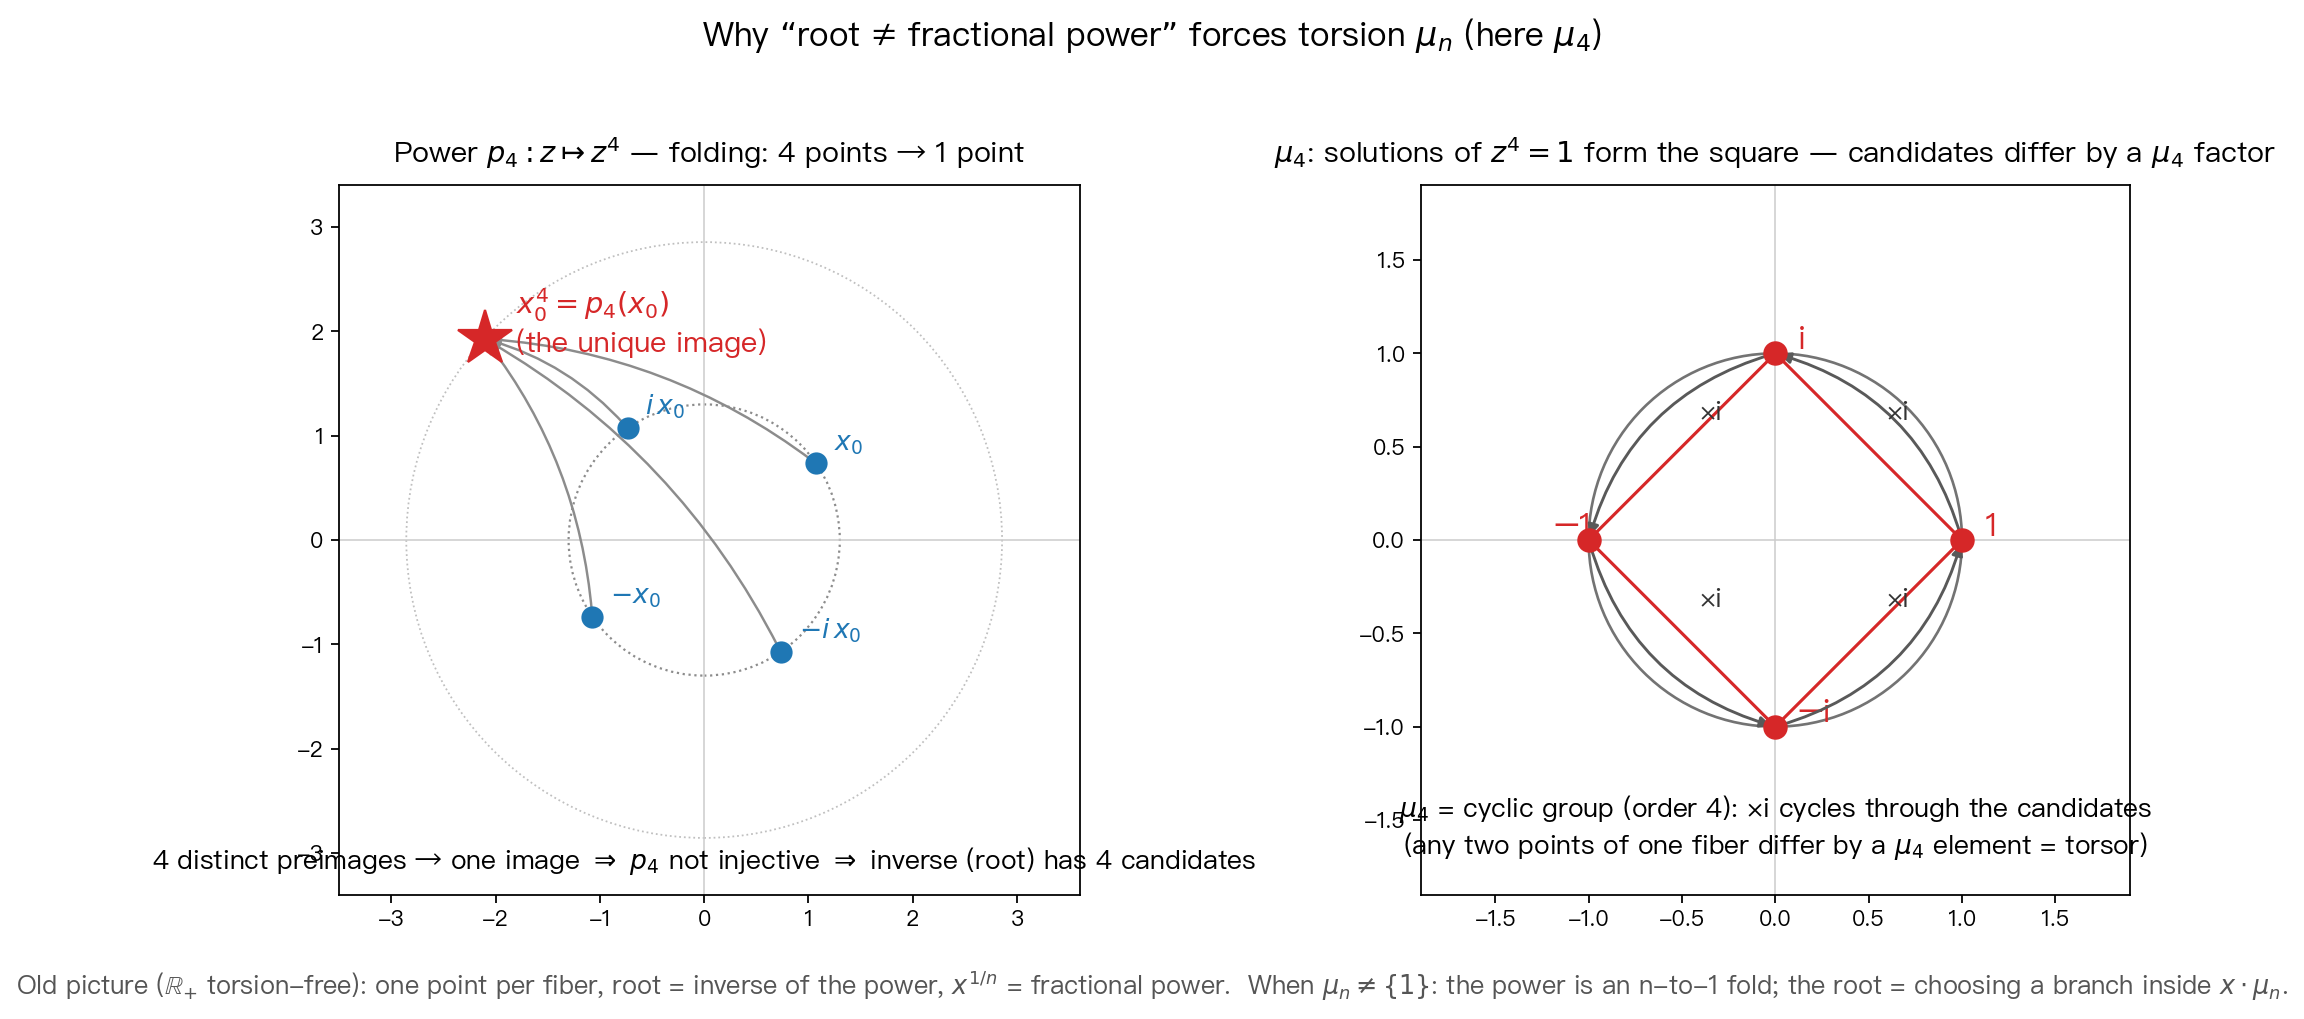
\includegraphics[width=0.9\textwidth]{root_vs_power_en}
\caption{Left: $p_4$ folds the four distinct points
$x_0,ix_0,-x_0,-ix_0$ of one fiber onto the single image $x_0^4$, so
the inverse problem ``which point maps here?'' has four answers, and the
radical is a choice among leaves rather than a value. Right: the four
leaves are not isolated; they form the coset $x_0\mu_4$ of the kernel
$\mu_4=\{1,i,-1,-i\}$ of $p_4$, and multiplication by $i$ cycles through
them, returning to the start after four steps. The power map identifies
a whole coset to one point, and the kernel acts freely and transitively
on the leaves above that point --- the torsor structure that a choice of
root must break.}
\label{fig:fold}
\end{figure}

\section{What torsion forces: explaining a number}\label{sec:numbers}

Two mechanisms are at work in what follows, and it is worth keeping
them apart. Whether a fiber is nonempty is an \emph{arithmetic}
question: over $\mathbb Q$ the equation $x^2=2$ has no solution at all
(machine-checked below), and the radical is forced into existence as a
new object rather than chosen as a symbol. When a fiber is nonempty,
its size is a \emph{torsion} question
(Corollary~\ref{cor:branches}): over $\mathbb R$ the two roots of
$x^2=2$ are $\pm\sqrt2$, which differ by $\mu_2=\{\pm1\}$. Existence is
arithmetic; multiplicity is torsion.
\begin{itemize}
\item no $n\in\mathbb N$ satisfies $n^2=2$ \Lean{two\_not\_sq\_nat};
\item no $q\in\mathbb Q$ satisfies $q^2=2$ \Lean{two\_not\_sq\_rat};
\item over the reals, $\sqrt 2$ exists and $(\sqrt2)^2=2$, and the
exponential/logarithm path gives the different exact formula
$e^{\ln 2}=2$.
\end{itemize}
The same number admits \emph{different} exact constructions, and which
families succeed depends on the number. Three families run through this
paper: pure powers ($25=5^2$), radicals ($\sqrt{25}=5$, an executable
integer square root), and exponential--logarithmic formulas
($\exp(\ln 25)=25$, the identity $\exp\circ\ln=\mathrm{id}$ on
$\mathbb R_+$). The number $2$ separates the first family from the other
two: no natural number and no rational number squares to $2$, so no
power formula explains it, and it is reached only once a radical object
is forced into existence. The golden section $\varphi$ is a radical
object in its own right: $\varphi=(1+\sqrt5)/2$ solves $x^2-x-1=0$, and
the verification is $\varphi^2=\varphi+1$.
Table~\ref{tab:exhibit} records the exhibit; an em dash marks the column
in which the family fails on that number.

\begin{table}[ht]
\centering
\begin{tabular}{lccc}
  & \emph{power} & \emph{radical} & \emph{exp--log}\\
  \hline
  $25$ & $25=5^2$ & $\sqrt{25}=5$ & $\exp(\ln 25)=25$\\
  $2$ & --- & $(\sqrt2)^2=2$ & $e^{\ln 2}=2$\\
  $\varphi$ & --- & $\varphi^2=\varphi+1$ & ---\\
  \hline
\end{tabular}
\caption{A number explained by whichever families succeed on it.
Entries are certified in the module or are direct instances of its
theorems (the identity $\exp\circ\ln=\mathrm{id}$ on $\mathbb R_+$); an
em dash marks a family that fails on that number.}
\label{tab:exhibit}
\end{table}

These are statements, not heuristics: the power claims are ring
computations, $\sqrt{25}=5$ is an executable integer reduction, and the
exponential--logarithmic claims are instances of the identity
$\exp\circ\ln=\mathrm{id}$. Each row is a different certified route
inside the same proof system.

\section{Certified radicals and a general quadratic solver}\label{sec:computation}

The examples of Section~\ref{sec:numbers} are instances of a general
solver. Fix real $b,c$ and the equation
\begin{equation}\label{eq:quad}
  x^2-bx-c=0,\qquad \Delta=b^2+4c .
\end{equation}

Whence the radicals. Completing the square exhibits the two roots
before they are named. From $x^2-bx-c=0$,
\begin{equation*}
  x^2-bx=\Bigl(x-\frac b2\Bigr)^2-\frac{b^2}{4}=c,
\end{equation*}
so that
\begin{equation*}
  (2x-b)^2=b^2+4c=\Delta.
\end{equation*}
Every root therefore satisfies the displayed identity, and conversely
any $x$ satisfying it is a root, by reversing the two steps. With
$\Delta\ge0$ the square root $\sqrt\Delta$ exists on $\mathbb R$, and
$2x-b=\pm\sqrt\Delta$ yields exactly the two candidates of
Theorem~\ref{thm:quad}. The failure direction is visible in the same
equation: when $\Delta<0$, the left side $(2x-b)^2$ is never negative.

\begin{theorem}[Quadratic radical solver]\label{thm:quad}
Let $\Delta=b^2+4c\ge 0$. Put
$r_+=(b+\sqrt\Delta)/2$ and $r_-=(b-\sqrt\Delta)/2$. Then
\begin{enumerate}
\item $r_+^2-br_+-c=0$ and $r_-^2-br_--c=0$;
\item for every $x$, $x^2-bx-c=(x-r_+)(x-r_-)$ --- there are no other
roots;
\item if $\Delta<0$ there is no real root at all.
\end{enumerate}
Consequently a real root exists if and only if $\Delta\ge 0$.
\end{theorem}
\begin{proof}
All claims are obtained by expanding and using
$(\sqrt\Delta)^2=\Delta$, which is the defining property of the real
square root; item~1 and item~2 are pure ring identities after that
substitution, and item~3 is completing the square:
$(2x-b)^2=\Delta$, impossible for $\Delta<0$.
\Lean{quadRootPlus\_sq, quadRootMinus\_sq, quadFactor, quad\_no\_roots,
quad\_solvable\_iff}
\end{proof}

Where the radicals come from. Cardano's substitution is a division of
labour between two unknowns. Put $x=u+v$ and impose $3uv=-p$; this is
one scalar condition on two degrees of freedom, and the leftover freedom
is exactly the $\mu_3$-torsor of Section~\ref{sec:quotient}: the pairs
$(u,v)$ and $(\zeta u,\zeta^{-1}v)$ satisfy the same condition for every
cube root of unity $\zeta$. Under the condition the cubic collapses:
\begin{align*}
  x^3+px+q &=(u+v)^3+p(u+v)+q\\
           &=u^3+v^3+(3uv+p)(u+v)+q
            =u^3+v^3+q ,\\
  u^3\,v^3 &=(uv)^3=(-p/3)^3=-p^3/27 .
\end{align*}
Hence $u^3$ and $v^3$ sum to $-q$ and multiply to $-p^3/27$: they are
the two roots of the auxiliary quadratic
\begin{equation*}
  z^2+qz-\frac{p^3}{27}=0,
\end{equation*}
whose discriminant is $\Delta_3=(q/2)^2+(p/3)^3$. If $\Delta_3\ge0$,
set $s=\sqrt{\Delta_3}$; the two auxiliary roots are $-q/2\pm s$, and
the theorem below builds a real root out of them. Note that $u$ must be
chosen among the three cube roots of $-q/2+s$ --- that freedom is the
$\mu_3$-torsor again --- and $v$ is then \emph{defined} from $u$ by
$v=-p/(3u)$, never chosen independently: an independent choice would let
$uv$ differ from $-p/3$ by a cube root of unity, and $u+v$ would fail to
be a root. Machine verification forces the definitional choice
\Lean{vcube, cardano\_certificate}.

\begin{theorem}[Cubic radical solution of Cardano]\label{thm:cubic}
Let $\Delta_3=(q/2)^2+(p/3)^3\ge 0$. Then $x^3+px+q=0$ has a real root,
constructed as follows. Put $s=\sqrt{\Delta_3}$, choose $u$ with
$u^3=-q/2+s$ (possible because the cube map is surjective on $\mathbb R$),
and set $v=-p/(3u)$. Then $v^3=-q/2-s$, $uv=-p/3$, and $u+v$ is a root.
\end{theorem}
\begin{proof}
$u^3+v^3=-q$ together with $3uv=-p$ gives
$(u+v)^3=u^3+v^3+3uv(u+v)=-q-p(u+v)$, hence $(u+v)^3+p(u+v)+q=0$.
The identity $v^3=-q/2-s$ follows from $(q/2)^2-s^2=-(p/3)^3$ and
$u\ne0$ by direct calculation (the case $u=0$ forces $p=0$, reducing to
$x^3+q$). Note that $v$ cannot be chosen as an \emph{independent} cube
root of $-q/2-s$: then $uv$ would differ by a cube root of unity --- the
third appearance of the torsion split of
Section~\ref{sec:quotient}, which machine verification forces us to face.
\Lean{cube\_surj, vcube, cardano\_certificate, cubic\_solvable}
\end{proof}

\textbf{Why $\exp$ and $\log$ here, and only here.} The formula
$\sqrt[n]{x}=\exp(\ln x/n)$ needs $\ln$ to be a single-valued function
and the collapse (1) to hold; both are true on $\mathbb R_+$, which is
torsion-free ($\mu_n(\mathbb R_+)=\{1\}$, Theorem~\ref{thm:collapse}).
Over $\mathbb C^\times$ the same formula would force $\ln$ to choose a
branch, and the branch choice is exactly a choice through $\mu_n$: the
exp/log route is the section written on the branch where the torsion is
invisible. That is why the construction is a statement about
$\mathbb R_+$, not about formula convenience.

\begin{theorem}[Radical of every degree]\label{thm:anydegree}
Let $n\ge 1$ be any degree and let $x>0$. On $\mathbb R_+$ the power map
$p_n$ is injective (Theorem~\ref{thm:collapse}: $\mu_n(\mathbb R_+)=\{1\}$),
and the unique positive solution $y$ of $y^n=x$ is
\begin{equation}\label{eq:anyroot}
y=\sqrt[n]{x}:=\exp\!\Big(\frac{\ln x}{n}\Big),
\end{equation}
with the following machine-checked consequences, for every $n\ge 1$:
\begin{enumerate}
\item $(\sqrt[n]{x})^n=x$;
\item if $a>0$ and $a^n=x$ then $a=\sqrt[n]{x}$ --- the radical is the
inverse of the power map, single-valued;
\item accordingly one formal statement covers every degree:
$n=2,3,5,\dots$ at once.
\end{enumerate}
The quintic makes the point: $(\sqrt[5]{32})^5=32$ and $\sqrt[5]{2^5}=2$
are instances of the same theorem as $\sqrt[3]{27}$ and $\sqrt{9}$; so is
$a^7=128 \Rightarrow a=\sqrt[7]{128}$. ``Roots of arbitrary degree'' here
means: for every natural degree simultaneously --- not a limit of a family
of functions as $n\to\infty$, but one theorem true for all $n$ at once.
\end{theorem}
\begin{proof}
By the definition, $(\sqrt[n]{x})^n=\exp(n\cdot\ln x/n)=\exp(\ln x)=x$,
which is item~1. For injectivity on $\mathbb R_+$, apply $\ln$ to
$a^n=b^n$: $n\ln a=n\ln b$, hence $\ln a=\ln b$ (division by $n\ne0$),
hence $a=b$ by exponentiation; item~2 combines this with item~1 and needs
no separate positivity hypothesis on $x$, since $a>0$ together with
$a^n=x$ already forces $x>0$.
\Lean{nthrootR\_pow, pow\_inj\_on\_Rpos, nthrootR\_eq\_of\_pow}
\end{proof}

The statements are machine-checked. Two boundaries are stated explicitly.

\begin{itemize}
\item \emph{Executability.} On $\mathbb N$ the integer square root
$\sqrt{25}=5$ is computed and reduced by the proof system itself
(\texttt{norm\_num}). On $\mathbb R$ the square root is defined by
completeness and is not executable; the reductions above (for example
$\sqrt{16}=4$ via $\sqrt{a^2}=\abs a$) are certified theorems, not
numeric iterations. We do not claim a numeric radical evaluator; we claim
certified radical statements.
\item \emph{The wall at degree five is a wall against mixed towers, not
against roots.} Pure $n$-th roots exist for every degree
(Theorem~\ref{thm:anydegree}); what dies at degree~5 is the
\emph{mixed} radical expression: the general quintic
$x^5+ax^4+bx^3+cx^2+dx+e=0$ is not solvable by any tower of field
operations and roots of arbitrary degree (Abel--Ruffini \citep{Abel1824});
stating that boundary precisely is the Galois half \citep{Galois1846} of
the programme and is not claimed here.
\end{itemize}

\section{Formalization notes}\label{sec:formal}

All statements marked with a Lean cross-reference above are proved in
Lean~4 \citep{deMoura2015} at version 4.21.0 with Mathlib
\citep{MathlibCommunity2020}, in the single module
\texttt{Nods.Theories.}\allowbreak\texttt{Radical} of the NODS repository,
imported by the main chain file \texttt{Nods.lean}. The proofs are short
--- Theorem~\ref{thm:ker} is definitional, Theorem~\ref{thm:fiber} is
one calculation in each direction, Theorem~\ref{thm:collapse} is an
instance of the standard kernel-trivial-iff-injective lemma --- and each
engineering choice below records an obstacle met while making those
proofs go through.
\begin{itemize}
\item \emph{Generic statements.} Every theorem is stated over an
arbitrary commutative group $G$ (\texttt{CommGroup}) rather than over
$\mathbb R_+$ alone, so the collapse criterion reads as a theorem about
torsion in any group and not as an accident of the positive reals --- a
choice that costs nothing, since the arguments use only commutativity
and the group laws.
\item \emph{An in-file kernel subgroup.} The roots of unity are built
in-file as \texttt{nRoots} $n\ G$, with carrier the set of $x$
satisfying $x^n=1$, rather than imported from Mathlib's units-based
\texttt{rootsOfUnity}; that library object lives on the unit group
(elements of $G^\times$ shipped with an inverse witness), while the
kernel of the power map is a plain subset of $G$, and coercing between
the two copies would buy nothing but transport lemmas at every use.
\item \emph{The power map is reused.} The map $p_n$ is not redefined:
the theorems use Mathlib's \texttt{powMonoidHom} directly, so
homomorphism facts, the kernel lemma, and the subgroup API apply to it
without glue.
\item \emph{Zero-\texttt{sorry}, zero-warning policy.} The module is
held to a strict standard: no \texttt{sorry} occurs in the source tree,
the module adds no \texttt{axiom} of its own, and the build is clean ---
``machine-checked'' refers to the checked-in file, not to a transcript
of a session.
\item \emph{The cube root is proved, not imported.} Surjectivity of the
cube map on $\mathbb R$ --- the analytic primitive behind the Cardano
step --- is proved in-system from Mathlib's intermediate value theorem
on a bounded interval (\texttt{intermediate\_value\_Icc}), because
Mathlib has no cube-root primitive; the IVT proof is the primitive
(Theorem~\ref{thm:cubic}).
\item \emph{Roots of every degree via $\exp$ and $\log$.} For arbitrary
degree no new primitive is built either: $\sqrt[n]{x}$ is defined as
$\exp(\ln x/n)$, and the two claims $(\sqrt[n]{x})^n=x$ and uniqueness
are derived from \texttt{exp\_nat\_mul} and \texttt{log\_pow} (via
injectivity of $\ln$ on $\mathbb R_+$), so one theorem covers every
$n\ge1$ at once (Theorem~\ref{thm:anydegree}).
\item \emph{Noncomputable reals, executable naturals.} Executability is
claimed only where it exists: \texttt{Real.sqrt}, \texttt{Real.exp},
\texttt{Real.log}, and the degree-$n$ root are noncomputable constants
fixed by real analysis, while \texttt{Nat.sqrt} is computable; the
executed examples are integer ones reduced by \texttt{norm\_num}
($\sqrt{25}=5$), whereas real identities such as $\sqrt{16}=4$ are
certified theorems derived from $\sqrt{a^2}=\abs a$, stated and proved
rather than computed.
\item \emph{Main-chain integration.} Integration is part of the claim:
the module is compiled in every full build of the repository through its
import by \texttt{Nods.lean}, so the formal content of this article is
exercised continuously rather than archived once.
\end{itemize}
As elsewhere in the paper, no number-theoretic conjecture is touched by
the module; the article's layout is inherited from an earlier preprint of
the author and carries none of its original mathematical content.

\section{Conclusion}\label{sec:conclusion}

The identification of the $n$-th root with a fractional power is not
false; it is local. Over $\mathbb C^\times$ the symbol $x^{1/n}$ names
one of $n$ candidates without saying which: power and radical are not
one operation wearing two names, but two structural roles --- a quotient
by $\mu_n$ and a section of the resulting $n$-fold cover --- and the
torsion subgroup $\mu_n$ is the exact measure of the difference, because
removing it collapses the distinction: $p_n$ becomes injective, and the
radical reverts to being the inverse of the power, precisely when
$\mu_n=\{1\}$ (Theorem~\ref{thm:collapse}). On $\mathbb R_+$ the
collapse is then no miracle of real analysis: $\mu_n\cap\mathbb R_+=\{1\}$,
the cover has nothing to be nontrivial over, and the section is a
function.

That the split is structural rather than rhetorical is the burden of the
certified ladder. The quadratic solver exhibits both roots of
$x^2-bx-c=0$ and factors the polynomial exactly when $\Delta\ge0$
(Theorem~\ref{thm:quad}); the Cardano construction exhibits a real root
of the depressed cubic and, in its proof, is forced to meet the torsion
split head-on, since $v$ may not be chosen as an independent cube root
of $-q/2-s$ (Theorem~\ref{thm:cubic}); and the pure $n$-th root then
flattens the ladder entirely, because one $\exp/\log$ statement yields
the unique positive root for every degree at once --- the quintic root
is not a further rung but the same theorem at $n=5$
(Theorem~\ref{thm:anydegree}).

The boundary of the claim is part of the claim. What dies at degree five
is not the root but the mixed tower: field operations closed under roots
of arbitrary degree solve every polynomial through degree four and fail
at the general quintic, and Abel--Ruffini and Galois theory
\citep{Abel1824,Galois1846} fix that boundary --- cited here rather than
proved, as they must be, since a formal proof is a separate programme,
not a missing paragraph. In the same spirit the real arithmetic
exhibited here is certified, not executed: integer radicals are computed
by the proof system (\texttt{norm\_num}), while statements such as
$\sqrt{16}=4$ are theorems about noncomputable constants, verified
through $\sqrt{a^2}=\abs a$; where the two regimes meet, the text states
the boundary explicitly.

\section{Further work}\label{sec:future}

None of the following is done; each item marks a boundary of the present
work rather than a claim.
\begin{itemize}
\item \emph{The complex full picture.} In $\mathbb C^\times$ one should
have $|\mu_n|=n$ and an $n$-valued root whose monodromy permutes the
branches by $\mu_n$, fusing the algebraic split of
Section~\ref{sec:quotient} with the analytic picture behind the
fractional-power notation. Cost: cyclotomic theory for
$\mu_n(\mathbb C^\times)$ together with covering-space machinery.
\item \emph{The formal Galois wall.} Proving --- rather than citing ---
Abel--Ruffini for the quintic inside Lean would make the boundary at
degree five internal to the system. Cost: solvable-group theory, field
extensions, and the insolubility of $S_5$ --- a large, separate
development.
\item \emph{Mixed-tower completions.} A translation step to the
depressed form for the general cubic, and Ferrari's quartic via its
cubic resolvent, would close the certified solvable range through degree
four. Cost: moderate, and the resolvent's root choices are the torsion
branch problems of Section~\ref{sec:quotient} again.
\item \emph{Certified numerical radicals.} Interval methods with
proof-carrying bounds would turn the certified but non-executable real
radicals of Section~\ref{sec:computation} into verified enclosures ---
a bridge from statements to computation. Cost: an approximation layer
for $\exp$, $\log$, and roots; substantial, but routine relative to this
development.
\end{itemize}

\bibliography{biblio}

\end{document}
